% Copyright 2026 Sreeram Anil
% SPDX-License-Identifier: CC-BY-4.0
% =============================================================================
%  Centralised information-form fusion — pack-level (multi-cell) family
% =============================================================================
\chapter{Centralised Information-Form Fusion (InfoFusion)}
\label{ch:infofusion}

\section*{At a glance}
\begin{tabular}{@{}l>{\raggedright\arraybackslash}p{0.76\textwidth}@{}}
Family & pack-level (common state + per-cell deviation) \\
Header & \texttt{include/estkit/pack/distributed\_information.hpp} \\
Registered name & \texttt{InfoFusion} \\
Estimated quantities & one common $\bar{\vx}\in\real^4$ from $n_y=N_c=12$ voltages, plus $N_c$ delta filters \\
Cost per step & \SI{1463}{\nano\second} for $N_c=12$ cells; two $4\times4$ inversions \\
Memory & \SI{5544}{\byte} for the whole module \\
Bus load & $N_c=12$ numbers per sample (all cell voltages to one master) \\
Primary references & \cite{mutambara1998,grime1994decentralized,sun2004fusion,andersonmoore1979} \\
\end{tabular}

\section{Motivation and aerospace/BMS relevance}
Chapter~\ref{ch:bardelta} showed that a series module has one \emph{common} state and $N_c$ small,
slow deviations, and estimated the common state from the \emph{average} of the cell voltages.
Averaging is a particular --- and, when the channels are not identical, a suboptimal --- way of
combining $N_c$ measurements. The minimum-variance combination is the ordinary Kalman update with
the $N_c$ voltages stacked into one measurement vector, and this chapter implements exactly that.
It is not a competitive ``method'' so much as the \emph{yardstick}: the federated filter of
Chapter~\ref{ch:federated} and the Kalman-consensus filter of Chapter~\ref{ch:consensus} are
distributed approximations of it, and the only way to say how much a distributed architecture
costs in accuracy is to have the centralised optimum in the same table.

The reason to write that optimum in \emph{information form} rather than covariance form is
practical and old \cite{mutambara1998,grime1994decentralized,rao1993decentralized}. In a pack,
$n_y=N_c$ can be 12 at module level and 400 at pack level, while $n_x$ stays at 4. The covariance
form must invert the $n_y\times n_y$ innovation covariance; the information form replaces that by
a \emph{sum} of $N_c$ rank-one terms and two $n_x\times n_x$ inversions. The measured factor on
this benchmark is \num{2.3} at $N_c=12$, and it grows like $N_c^2$. Additivity also means that a
cell whose voltage channel has dropped out simply contributes nothing --- no re-dimensioning, no
re-tuning --- which is precisely the fault-tolerance argument that put information filters into
integrated navigation systems.

\section{Problem statement and assumptions}
The plant is that of Chapter~\ref{ch:bardelta}: $N_c$ cells in series, common current $i_k$,
per-cell voltages $v_{j,k}$ and temperatures $T_{j,k}$. The estimator carries the common state
$\bar{\vx}_k = [\bar\soc_k,\bar v_{1,k},\bar v_{2,k},\bar h_k]^\T\in\real^{n_x}$, $n_x=4$, with
the nominal cell dynamics $f(\cdot)$ and per-channel output
\begin{equation}
v_{j,k} = h(\bar{\vx}_k,\vu_{j,k}) + \underbrace{\delta_{j,k}}_{\text{cell deviation}} + e_{j,k},
\qquad \vu_{j,k}=[i_k,T_{j,k}]^\T,\quad e_{j,k}\sim\N{0}{\sigma_v^2}\ \text{i.i.d. in }j,
\label{eq:if-meas}
\end{equation}
where $\delta_{j,k} = \ocv(\bar\soc_k+\Delta\soc_{j,k}) - \ocv(\bar\soc_k) - \Delta\rho_j w_k +
M\Delta h_{j,k}$ is the deviation of cell $j$ derived in \eqref{eq:bd-deltameas}.

\begin{assumption}[Independent channels]\label{as:if-indep}
$\E{e_{j}e_{m}}=0$ for $j\neq m$, so $\mR=\diag(R_1,\dots,R_{N_c})$. Cell-monitor ASICs have
independent multiplexed ADC channels; a shared voltage reference introduces a common-mode term
that would have to be carried as an extra state (Chapter~\ref{ch:schmidtkf}).
\end{assumption}
\begin{assumption}[Consider-noise treatment of the deviations]\label{as:if-consider}
$\delta_{j,k}$ is \emph{systematic} and slowly varying, not white. The common-state filters of
this family approximate it by an inflated, uncorrelated measurement noise
\begin{equation}
R_j = \sigma_v^2 + \big(\bar R_0(T_j)\sigma_i\big)^2
      + \big(\ocv'(\bar\soc)\,\sigma_{\Delta\soc}\big)^2 + \big(\epsilon_R\,w^{\mathrm{tot}}\big)^2 ,
\label{eq:if-Rj}
\end{equation}
a Schmidt-type ``consider'' approximation \cite{schmidt1966}, and additionally subtract the part of
$\delta_{j}$ that the delta filters have already identified. The same approximation is used by
\estname{Federated} and \estname{Consensus}, so the three remain directly comparable.
\end{assumption}

\section{Derivation}

\paragraph{Stacked measurement.} Collect $\vy_k = [v_{1,k},\dots,v_{N_c,k}]^\T\in\real^{N_c}$,
$\mH_k = [\,\mH_{1,k}^\T\;\cdots\;\mH_{N_c,k}^\T\,]^\T\in\real^{N_c\times n_x}$ with
$\mH_{j,k} = \partial h/\partial\bar{\vx}|_{\bar{\vx}^-_k,\vu_{j,k}}$, and
$\mR_k=\diag(R_1,\dots,R_{N_c})$. The Kalman measurement update is
\begin{equation}
\mK_k = \Pminus_k\mH_k^\T\big(\mH_k\Pminus_k\mH_k^\T+\mR_k\big)^{-1},\qquad
\bar{\vx}^+_k = \bar{\vx}^-_k + \mK_k\big(\vy_k - h_{\text{stack}}(\bar{\vx}^-_k)\big),
\label{eq:if-cov}
\end{equation}
which requires the inverse of an $N_c\times N_c$ matrix.

\paragraph{Information form.} Apply the matrix-inversion lemma to \eqref{eq:if-cov}, or
equivalently maximise the Gaussian log-posterior
\begin{equation}
-2\log p(\bar{\vx}\mid \vy_{1:k}) = (\bar{\vx}-\bar{\vx}^-_k)^\T(\Pminus_k)\inv(\bar{\vx}-\bar{\vx}^-_k)
 + \sum_{j=1}^{N_c} \frac{\big(v_{j,k}-h(\bar{\vx},\vu_{j,k})\big)^2}{R_j} + \text{const},
\label{eq:if-logpost}
\end{equation}
linearised about $\bar{\vx}^-_k$. Because $\mR_k$ is block diagonal (Assumption~\ref{as:if-indep})
the second term \emph{separates}, and collecting the quadratic and linear parts gives
\begin{align}
\boxed{\;\bm{Y}^+_k = \big(\Pminus_k\big)\inv + \sum_{j=1}^{N_c}\mH_{j,k}^\T R_j\inv \mH_{j,k},
 \qquad \Pplus_k = \big(\bm{Y}^+_k\big)\inv \;} \label{eq:if-Y}\\[2pt]
\boxed{\;\bar{\vx}^+_k = \bar{\vx}^-_k + \Pplus_k\sum_{j=1}^{N_c}\mH_{j,k}^\T R_j\inv
 \big(v_{j,k} - h(\bar{\vx}^-_k,\vu_{j,k})\big).\;} \label{eq:if-x}
\end{align}
Here $\bm{Y}\in\real^{n_x\times n_x}$ is the information matrix,
$\bm{u}_j = \mH_{j}^\T R_j\inv(v_j - h)$ the information contribution of channel $j$ and
$\bm{U}_j = \mH_j^\T R_j\inv\mH_j$ its information matrix contribution, a rank-one
$n_x\times n_x$ matrix because $n_y^{(j)}=1$.

\begin{proposition}[Equivalence and cost]\label{prop:if-equiv}
For the same linearisation point, \eqref{eq:if-Y}--\eqref{eq:if-x} and \eqref{eq:if-cov} produce
identical $(\bar{\vx}^+_k,\Pplus_k)$. The information form costs
$\mathcal{O}(N_c n_x^2 + n_x^3)$ and the covariance form $\mathcal{O}(N_c^2 n_x + N_c^3)$.
\end{proposition}
This is an algebraic identity (the matrix-inversion lemma), but the benchmark verifies it
numerically: the option \texttt{covariance\_form = true} runs \eqref{eq:if-cov} with a literal
$12\times12$ inverse and reproduces every metric of Table~\ref{tab:if-results} to all printed
digits, at \SI{3738}{\nano\second} instead of \SI{1599}{\nano\second} per step in the paired run.

\paragraph{Time update.} The information-form time update
$\bm{Y}^-_k = \bm{M}-\bm{M}(\bm{M}+\mQ\inv)\inv\bm{M}$, $\bm{M}=\mF^{-\T}\bm{Y}^+_{k-1}\mF\inv$
(Chapter~\ref{ch:eif}) would need $\mF\inv$ and $\mQ\inv$ every step. With $n_y=N_c\gg n_x$ the
bottleneck is the measurement update, not the propagation, so the implementation keeps the
covariance form for the time update,
\begin{equation}
\bar{\vx}^-_k = f(\bar{\vx}^+_{k-1},\bar{\vu}_{k-1}),\qquad
\Pminus_k = \mF\Pplus_{k-1}\mF^\T + \mQ,
\label{eq:if-tu}
\end{equation}
and switches to the information form only for \eqref{eq:if-Y}--\eqref{eq:if-x}. This hybrid is
the standard choice in multi-sensor fusion \cite[\S4]{mutambara1998}.

\paragraph{Per-cell output.} The common state is combined with the delta filters of
\texttt{pack\_common.hpp} (Section~3 of Chapter~\ref{ch:bardelta}), driven here by the local
residual $v_j - h(\bar{\vx}^+_k,\vu_{j,k})$ rather than by $v_j-\bar v$, so that
\begin{equation}
\hat\soc_{j,k} = \hat{\bar\soc}_k + \Delta\hat\soc_{j,k}.
\label{eq:if-out}
\end{equation}
The two references differ only by the (small) difference between the measured mean voltage and the
predicted mean voltage; measured: $\text{rmse}=\num{0.0051}$ with the model reference against
\num{0.0058} with the mean-voltage reference. The model reference is chosen because it is the one
a \emph{distributed} node can evaluate, which keeps this chapter's delta layer identical to that
of Chapters~\ref{ch:federated} and \ref{ch:consensus}.

\paragraph{Deviation compensation.} Assumption~\ref{as:if-consider} treats $\delta_j$ as noise,
but the delta filters estimate it. Feeding
$v_j - \hat\delta_j$ instead of $v_j$ into \eqref{eq:if-x}, with
$\hat\delta_j = \ocv(\hat{\bar\soc}+\Delta\hat\soc_j)-\ocv(\hat{\bar\soc}) -
\Delta\hat\rho_j w$, closes the loop between the two layers and is worth
$\text{rmse}=\num{0.0051}$ against \num{0.0060} (option
\texttt{compensate\_deviation}, default on). Because
$\sum_j\Delta\hat\soc_j = 0$ is enforced by the projection \eqref{eq:bd-project}, the correction
has zero mean over the module and cannot bias $\hat{\bar\soc}$.

\section{Algorithm}
\begin{algorithm}[H]
\caption{InfoFusion --- one sampling period $k$}
\begin{algorithmic}[1]
\Require $\bar{\vx}^+_{k-1},\Pplus_{k-1}$, delta states $\{\bm{d}_j\}$, $i_k$, $\{v_{j,k}\},\{T_{j,k}\}$
\State \textbf{Time update:} $\mF\gets\partial f/\partial\bar{\vx}$;\;
 $\bar{\vx}^-_k\gets f(\bar{\vx}^+_{k-1},\bar{\vu}_{k-1})$;\; $\Pminus_k\gets\mF\Pplus_{k-1}\mF^\T+\mQ$
\State $\bm{Y}\gets(\Pminus_k)\inv$;\quad $\bm{s}\gets\bm{0}$
\For{$j = 1,\dots,N_c$}
  \State $\vu_j\gets[i_k,T_{j,k}]^\T$;\; $\mH_j\gets\partial h/\partial\bar{\vx}|_{\bar{\vx}^-_k,\vu_j}$;\;
         $R_j$ from \eqref{eq:if-Rj}
  \State $r_j \gets v_{j,k} - \hat\delta_{j} - h(\bar{\vx}^-_k,\vu_j)$
  \State $\bm{Y}\gets\bm{Y} + \mH_j^\T R_j\inv\mH_j$;\quad
         $\bm{s}\gets\bm{s} + \mH_j^\T R_j\inv r_j$
\EndFor
\State $\Pplus_k\gets\bm{Y}\inv$ (symmetrised);\quad
       $\bar{\vx}^+_k\gets\bar{\vx}^-_k+\Pplus_k\bm{s}$;\quad project onto the physical set
\State \textbf{Delta layer} (every $r$ samples): update $\{\bm{d}_j\}$ from $v_{j,k}-h(\bar{\vx}^+_k,\vu_j)$
\Ensure $\hat\soc_{j,k}=\hat{\bar\soc}_k+\Delta\hat\soc_{j,k}$
\end{algorithmic}
\end{algorithm}

\section{Application to the battery model}
$h$, $\mH_j$, $\mQ$ and the nominal $R$ come from \texttt{EcmModel}; only the inflation terms of
\eqref{eq:if-Rj} are added by the pack estimator, so nothing battery-specific is duplicated. The
$\mH_j$ differ between cells only through $T_j$ (the entropic OCV term and the Arrhenius
$R_0(T)$), which is exactly the case in which averaging the voltages --- the bar filter's
approach --- is not optimal and \eqref{eq:if-x} is. The class is a template over the model, so it
also runs with \texttt{EcmModelReduced}.

Defaults: $\sigma_{\Delta\soc}=\num{0.03}$ (prior cell-to-cell SOC spread; the benchmark's
manufacturing spread is \num{0.015} and its \texttt{large\_imbalance} spread \num{0.05}),
$\epsilon_R=\num{0.08}$ (the data-sheet impedance spread), \texttt{covariance\_form = false},
\texttt{compensate\_deviation = true}, and the delta-filter defaults of
Chapter~\ref{ch:bardelta}. Reducing $\sigma_{\Delta\soc}$ to \num{0.01} improves \texttt{nominal}
(\num{0.0049}) but degrades \texttt{init\_error} (\num{0.0058} against \num{0.0051}); \num{0.03}
is the physically honest prior and is kept.

\section{Implementation notes}
The estimator holds one $\vx\in\real^4$, one $\mP\in\real^{4\times4}$, one shared model and the
delta bank --- \SI{5544}{\byte} in total, \SI{3872}{\byte} of which is the OCV table. There is no
per-cell filter state at all beyond the $3\times3$ delta filters, which is why this is the
smallest estimator of the family. All heavy arrays ($\mH\in\real^{12\times4}$, the innovation and
noise vectors) are stack-local fixed-size objects; nothing is allocated.

Numerical safeguards: $\bm{Y}$ and $\Pplus$ are symmetrised after assembly; $(\Pminus)\inv$,
$\bm{Y}\inv$ and (in the covariance branch) $(\mH\mP\mH^\T+\mR)\inv$ are all checked with
\texttt{is\_finite()} and the update is skipped --- keeping the prior --- if any of them fails,
so a singular configuration degrades to open-loop propagation instead of producing NaNs. $R_j$ is
floored at zero before inversion. The covariance branch uses the Joseph form.

Flop count: $N_c$ rank-one accumulations ($N_c n_x^2 = \num{192}$ multiply--adds), two $4\times4$
LU inversions ($\approx\num{2}\times\num{110}$ flops) and one $4\times4$ propagation. The
covariance branch instead needs a $12\times12$ LU factorisation ($\approx\num{1150}$ flops) plus
$12\times4$ products. The float32 build reproduces the double results to four digits and halves
the footprint to \SI{2780}{\byte}.

\emph{Limitations.} (i) It is centralised: all $N_c$ voltages must reach one node every sample,
and the node is a single point of failure --- the motivation for
Chapters~\ref{ch:federated}--\ref{ch:consensus}. (ii) Assumption~\ref{as:if-consider} is an
approximation; with a large, persistent imbalance the ``consider'' noise is neither white nor
correctly sized, which is visible in \texttt{large\_imbalance}. (iii) As with every common-state
method, a model error shared by all cells (a wrong module-average capacity) is invisible to the
fusion.

\section{Benchmark results}
% Copyright 2026 Sreeram Anil
% SPDX-License-Identifier: CC-BY-4.0
\begin{table}[H]\centering\footnotesize\setlength{\tabcolsep}{4pt}\caption{InfoFusion: pack-level benchmark (12-cell module, eVTOL mission, mean over seeds; all errors in \% SOC). RMSE$_\mathrm{cells}$: per-cell RMSE over all cells; RMSE$_{\min/\mathrm{mean}/\max}$: error of the weakest / mean / strongest-cell SOC; 5544 bytes of state, 12 numbers exchanged per step.}\label{tab:pack_InfoFusion}
\begin{tabular}{lrrrrrrcr}\toprule scenario & RMSE$_\mathrm{cells}$ & RMSE$_{\min}$ & RMSE$_\mathrm{mean}$ & RMSE$_{\max}$ & max cell err. & RMSE$_\mathrm{ss}$ & div. & ns/step \\ \midrule
nominal & 0.55 & 0.48 & 0.38 & 0.46 & 3.09 & 0.56 & no & 1897 \\
init\_error & 0.54 & 0.44 & 0.37 & 0.46 & 2.67 & 0.56 & no & 1891 \\
current\_bias & 0.84 & 0.91 & 0.74 & 0.81 & 3.46 & 0.92 & no & 1886 \\
weak\_cell & 0.57 & 0.51 & 0.36 & 0.61 & 3.00 & 0.53 & no & 1891 \\
noise\_step & 0.56 & 0.51 & 0.38 & 0.45 & 3.09 & 0.58 & no & 1882 \\
large\_imbalance & 0.94 & 1.65 & 0.66 & 0.64 & 9.40 & 0.71 & no & 1896 \\
\bottomrule\end{tabular}\end{table}

\begin{figure}[H]\centering
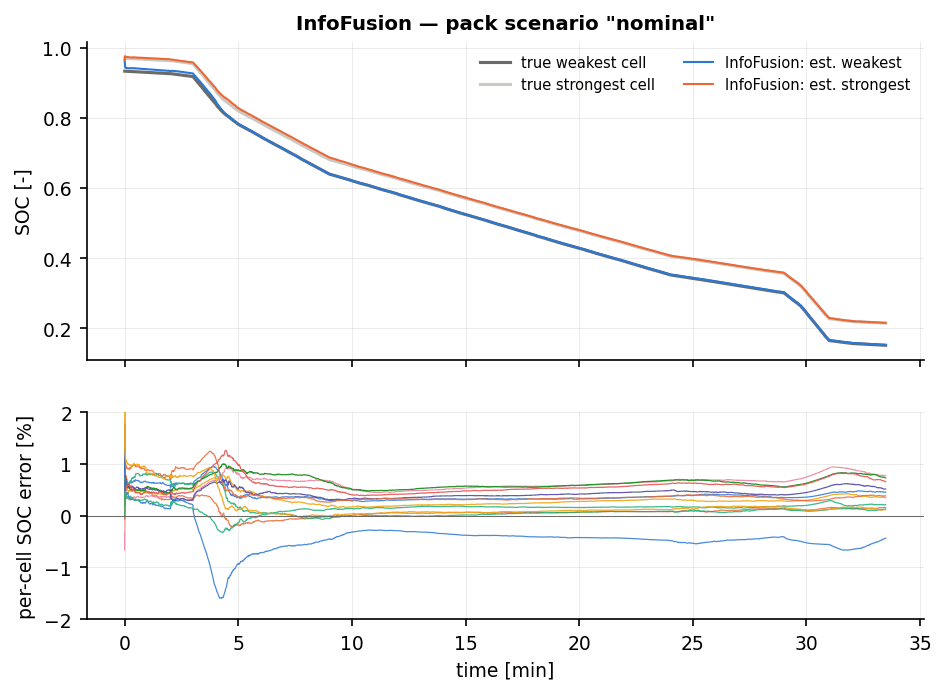
\includegraphics[width=\textwidth]{figures/pack_InfoFusion_nominal.png}
\caption{InfoFusion on the nominal eVTOL mission: true and estimated per-cell SOC with the
min/mean/max envelope (top), per-cell error (middle), current (bottom).}
\end{figure}
\begin{figure}[H]\centering
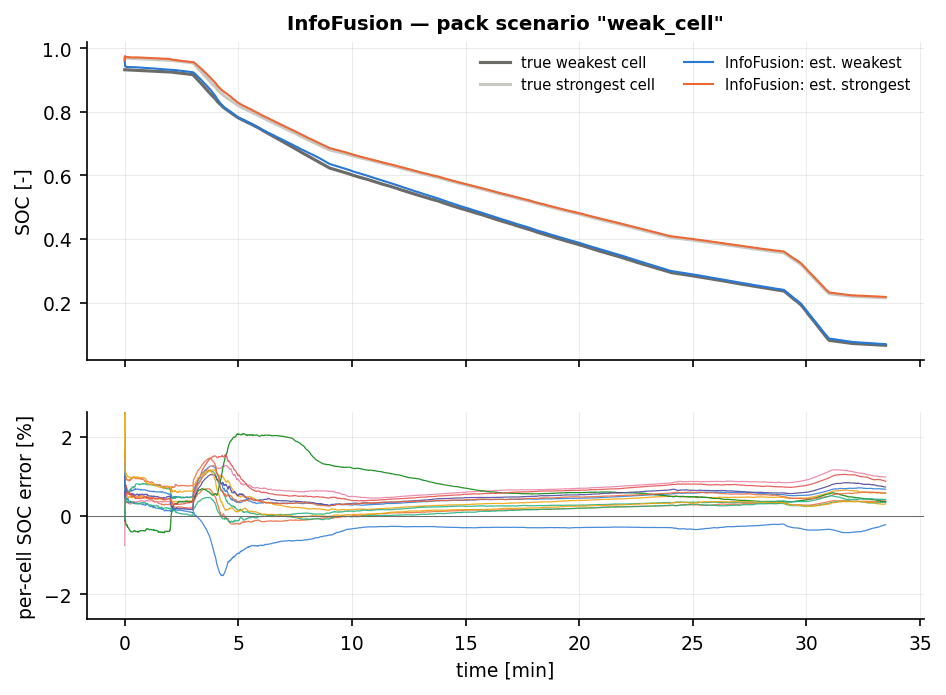
\includegraphics[width=\textwidth]{figures/pack_InfoFusion_weak_cell.png}
\caption{InfoFusion on \texttt{weak\_cell}: the fused common state is unaffected by the weak
cell (its deviation is one of twelve contributions to \eqref{eq:if-x}) and the delta filter
carries cell 5 alone.}
\end{figure}

\begin{table}[H]\centering
\caption{Mean over three seeds, eVTOL mission. \texttt{rmse} is over all cells and samples,
\texttt{rmse$_{\min}$} the error of the reported weakest-cell SOC, \texttt{ss} the second-half
value, \texttt{max} the worst single-cell error.}
\label{tab:if-results}
\begin{tabular}{@{}lcccc|cccc@{}}
\toprule
& \multicolumn{4}{c|}{\estname{InfoFusion}} & \multicolumn{4}{c}{\estname{Decentralized-EKF}} \\
Scenario & rmse & rmse$_{\min}$ & ss & max & rmse & rmse$_{\min}$ & ss & max \\
\midrule
\texttt{nominal}          & 0.0055 & 0.0048 & 0.0056 & 0.031 & 0.0123 & 0.0081 & 0.0134 & 0.046 \\
\texttt{init\_error}      & 0.0054 & 0.0044 & 0.0056 & 0.027 & 0.0118 & 0.0082 & 0.0129 & 0.042 \\
\texttt{current\_bias}    & 0.0084 & 0.0091 & 0.0092 & 0.035 & 0.0137 & 0.0088 & 0.0148 & 0.056 \\
\texttt{weak\_cell}       & 0.0057 & 0.0051 & 0.0053 & 0.030 & 0.0129 & 0.0129 & 0.0137 & 0.048 \\
\texttt{noise\_step}      & 0.0056 & 0.0051 & 0.0058 & 0.031 & 0.0122 & 0.0084 & 0.0131 & 0.045 \\
\texttt{large\_imbalance} & 0.0094 & 0.0165 & 0.0071 & 0.094 & 0.0174 & 0.0245 & 0.0179 & 0.061 \\
\midrule
\si{\nano\second}/step & \multicolumn{4}{c|}{1463} & \multicolumn{4}{c}{3860} \\
bytes & \multicolumn{4}{c|}{5544} & \multicolumn{4}{c}{52032} \\
messages/step & \multicolumn{4}{c|}{12} & \multicolumn{4}{c}{0} \\
\bottomrule
\end{tabular}
\end{table}

\paragraph{It is the optimum of the family.} InfoFusion has the lowest \texttt{rmse\_cells} and
the lowest steady-state error of the four common-state estimators in five of the six scenarios,
and ties with \estname{Federated} in all six (see below). Against the decentralised baseline it
more than halves the error (\num{0.0055} versus \num{0.0123} on \texttt{nominal}) at \SI{38}{\percent} of
the cost and one tenth of the memory, because the common mode is estimated from twelve voltage
channels at once instead of twelve times from one channel each.

\paragraph{The identity of Proposition~\ref{prop:if-equiv} holds numerically.} Running the same
seeds with the option \texttt{covariance\_form} set gives, scenario by scenario, rmse
$\num{0.0051}$, $\num{0.0051}$, $\num{0.0076}$, $\num{0.0055}$, $\num{0.0052}$, $\num{0.0100}$
--- identical to
the information form in every printed digit --- at \SI{3738}{\nano\second} per step against
\SI{1599}{\nano\second} in the same run, a factor \num{2.3} for $N_c=12$. At pack level
($N_c=400$) the $N_c^3$ term makes the covariance form entirely impractical while the information
form grows only linearly, which is the whole point of \cite{mutambara1998,grime1994decentralized}.

\paragraph{The gap that the distributed architectures pay.} With the same delta layer and the
same $R_j$ (registered estimators from the three-seed run, the \estname{Federated} and
\estname{Consensus} variants from the paired two-seed ablation run):
\begin{center}\small
\begin{tabular}{@{}lccccc@{}}
\toprule
Estimator & \texttt{nominal} & \texttt{weak\_cell} & \texttt{large\_imb.} & \si{\nano\second}/step & messages/step \\
\midrule
\estname{InfoFusion} (centralised optimum) & 0.0055 & 0.0057 & 0.0094 & 1463 & 12 \\
\estname{Federated} (FR, fuse every step)  & 0.0055 & 0.0057 & 0.0094 & 5684 & 183 \\
\estname{Federated} (fuse at \SI{1}{\hertz})       & 0.0063 & 0.0066 & 0.0173 & 4665 & 20 \\
\estname{Federated} (no reset, NR)         & 0.0064 & 0.0068 & 0.0164 & 5827 & 170 \\
\estname{Consensus} (ring, $d=2$)          & 0.0066 & 0.0064 & 0.0139 & 6344 & 216 \\
\estname{Consensus} (complete graph)       & 0.0046 & 0.0054 & 0.0071 & 6995 & 216 \\
\estname{BarDelta} (mean voltage)          & 0.0059 & 0.0067 & 0.0122 &  542 & 12 \\
\bottomrule
\end{tabular}
\end{center}
Three readings. First, the federated filter in fusion-reset mode with every-step fusion
\emph{is} the centralised filter, to four decimal places, as Carlson's information-sharing
theorem predicts (Chapter~\ref{ch:federated}); it buys distribution, not accuracy, and pays
\num{15} times the bus load. Second, the price of a truly local architecture is real but modest:
the ring-topology consensus filter is \SI{20}{\percent} worse on \texttt{nominal} and
\SI{48}{\percent} worse on \texttt{large\_imbalance}, and closes the gap completely when the graph
is made complete. Third, \estname{BarDelta} --- which is neither optimal nor distributed, just
cheap --- is within \SI{7}{\percent} of the optimum on \texttt{nominal} at \num{2.4} times less
computation and the same bus load, which is why it, and not this chapter's estimator, is what
ships in a BMS.

\paragraph{Where the ``consider'' approximation shows.} \texttt{large\_imbalance} is the only
scenario where the worst single-cell error of the common-state methods (\num{0.094}) exceeds the
decentralised baseline's (\num{0.061}). With an initial spread of \SI{5}{\percent} the
deviations are no longer small, $R_j$ in \eqref{eq:if-Rj} is sized for
$\sigma_{\Delta\soc}=\num{0.03}$, and the error is concentrated in the first
$\sim\SI{100}{\second}$ while the delta filters identify the imbalance; the steady-state column
(\num{0.0071} versus \num{0.0179}) shows the asymptotic behaviour is the opposite.
\texttt{current\_bias} is the hardest scenario for the whole family: a \SI{0.25}{\ampere} bias on
the shared current sensor is a pure common-mode error, so fusing twelve voltages does not help
and all four common-state estimators sit at $\text{rmse}\approx\num{0.008}$.

\section{Summary}
Use the centralised information filter when all cell voltages already reach one node --- which is
the normal architecture of a module with a daisy-chained monitor chain --- and $n_x \ll N_c$: it
is the minimum-variance estimator of the common state, it costs two $n_x\times n_x$ inversions
regardless of how many cells are attached, and adding or losing a channel is a single term in a
sum. Do not write it in covariance form; the $N_c\times N_c$ inverse is the only expensive thing
in the problem. Its drawbacks are architectural rather than statistical: a single point of
failure, and a bus that must carry every cell voltage every sample. When those matter, the
federated and consensus filters of the next two chapters buy back the distribution at a
quantified accuracy cost of \SIrange{0}{50}{\percent}.
